\section{Method}
This section explains how the implementation was done and how the experiments were conducted. After that follows an outline of the experiment setup and a discussion of the experiments.
\subsection{Implementation}
Implementation was done using two libraries and several books to make a corpus. KYLM\footnote{A full list of resources can be found in section \ref{sec:resources}} was a library that had several smoothing techniques implemented. We used it to process our corpus and make an arpa-file, consisting of n-grams of different sizes and their probability derived from the corpus and chosen smoothing technique. We also used OpenNLP, a part-of-speech-tagger that we could use in the implementation of grammar constraints in the word predictor. The rest of the program: searching the arpa-files, grammar constraints, context recognition and user interface was implemented by the authors.\\

To test our hypotheses, a qualitative inductive method was used. Evaluation and comparison of the different functionalities was made by measuring keystroke counts. This seemed to be a widely used method, and suited our project as it is an objective performance evaluation, and user interface/experience was of no interest for the study.\\

In a keystroke count experiment, for a given word, the number of keystrokes are the number of keys that the participant has to press in order for the word predictor to suggest the word the participant meant to write. In this experiment, given previous words, the word predictor may be able to suggest the thought of word without any strokes in which case the keystroke count for that word is zero. Spaces between words did not count as keystrokes.

\subsection{Evaluation}
Four sentences that were thought to bring out the differences in the different functionalities were constructed. 
\begin{figure}[h]
\center
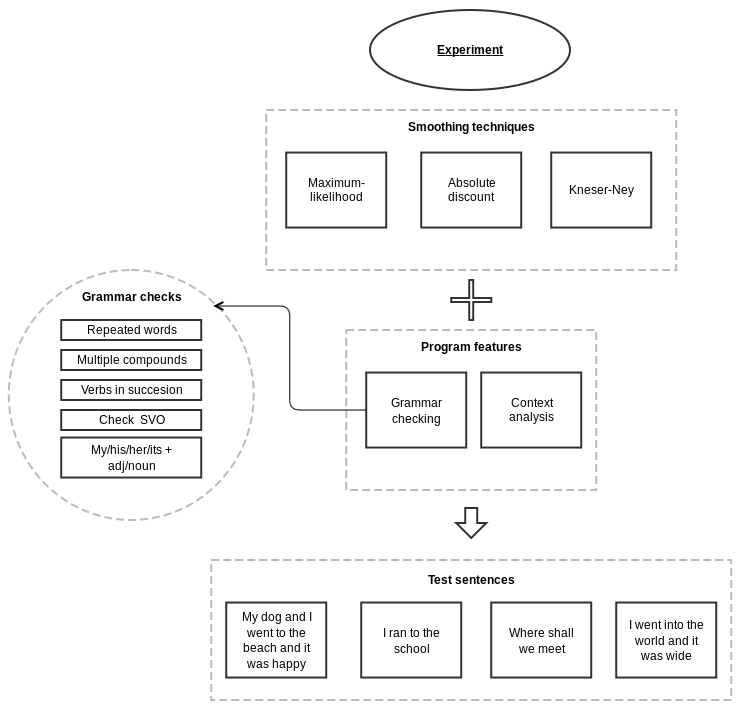
\includegraphics[width=0.7\textwidth]{img/experiment_diagram.png}
\label{fig:experiments}
\caption{Diagram showing how experiments were conducted}
\end{figure}
Tests were then performed for each sentence, for each combination of functionalities and for each smoothing technique, which made a total of 48 different tests. From here follows a more detailed description of the evaluation and the experiment parameters.
\subsection{Experimental setup}
\lipsum[1]